\section{9/19/2019}

\subsection{Recap}

\begin{itemize}
  \item Expand $\cG$ to $\cM$
    \begin{itemize}
      \item Bound modulus of $\cM$
      \item Show $p_n^* \in \cM$
      \item Bound $\|\mu(p_n^*) - \mu(p^*)\|_2$
    \end{itemize}
  \item $\cG = \cG_k(\sigma) =$ bounded $k$th moments
    (needed $n \geq d^{k/2}$ samples if $\cM = \cG$)
  \item $\cM = \cG_{\TV}(\rho, \eps) =$ $(\rho, \eps)$-resilient distributions
    with $\rho = \cO(\sigma \eps^{1 - 1/k})$
\end{itemize}

\subsection{Truncated moments bounds}

Our strategy to show $p_n^* \in \cM$ is to consider the truncated (Orlicz)
function
\begin{align}
  \tilde{\psi}_k &= \begin{cases}
    x^k &\text{if } x \leq x_0 \\
    k x_0^{k-1} (x - x_0) + x_0^k&\text{if } x > x_0
  \end{cases}
\end{align}
This function behaves as $x^k$ until $x=x_0$, after which it is linear.
See \cref{fig:tilde-psi-k}.
Note that $\tilde{\psi}_k$ is $L$-Lipschitz with $L = k x_0^{k-1}$.

\textbf{Todo this lecture:}
\begin{itemize}
  \item Ledoux-Talagrand
  \item Bound $\|\mu(p_n^*) - \mu(p^*)\|_2$ via Khintchine and Rosenthal
  \item Show truncated moments $\tilde{\psi}$ concentrate
\end{itemize}

\begin{definition}[Stochastic Dominance]
  Let $Y, Z$ be RVs on $\RR$.
  $Z$ \emph{1st-order stochastically dominates} $Y$,
  denoted by $Z \succeq_1 Y$, if
  \begin{align}
    \ex[f(Z)] \geq \ex[f(Y)]
  \end{align}
  for all increasing $f$.

  \begin{figure}[H]
    \begin{center}
      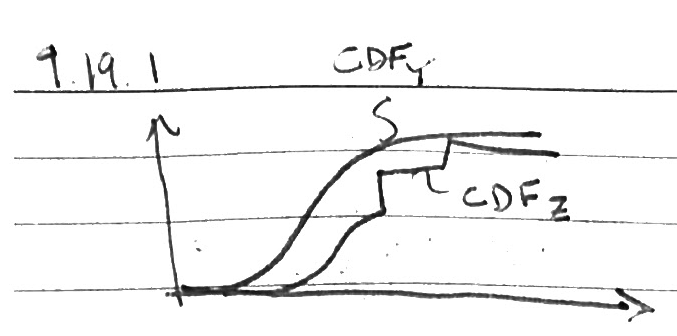
\includegraphics[width=0.4\textwidth]{figures/9-19-1.png}
    \end{center}
    \caption{Intuition for $Z \succeq_1 Y$: going from $Y$ to $Z$ shifts
    cumulative distribution function (CDF) to the right}
  \end{figure}
\end{definition}

\begin{lemma}[Two-point first order stochastic dominance]
  For $y_1 \leq y_2$ and $z_1 \leq z_2$, let
  \begin{align}
    Y &\sim \frac{1}{2} \delta_{y_1} + \frac{1}{2} \delta_{y_2} \\
    Z &\sim \frac{1}{2} \delta_{z_1} + \frac{1}{2} \delta_{z_2}
  \end{align}
  Then $Z \succeq_1 Y$ iff $y_1 \leq z_1$
  and $y_2 \leq z_2$.
\end{lemma}

\begin{proof}
  For the necessity, consider $f_\tau(x) = \ind\{x \geq \tau\}$ a step function.
  \begin{figure}[H]
    \begin{center}
      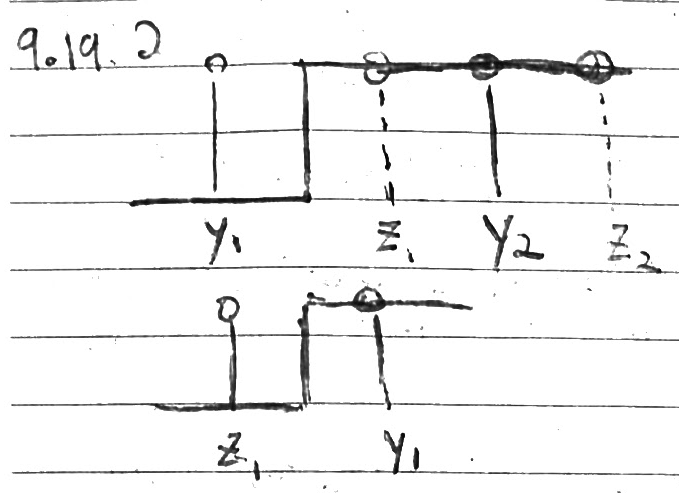
\includegraphics[width=0.5\textwidth]{figures/9-19-2.png}
    \end{center}
  \end{figure}
  A violation of $y_1 \leq z_1$ and $y_2 \leq z_2$ would imply for some $\tau$ both
  of the $y_i \leq \tau$ but only $z_1 \leq \tau$. The increasing function $f_\tau$
  gives a contradiction to $Z \succeq_1 Y$, as
  \begin{align}
    \ex[f_\tau(Y)] = 1 \not\leq \frac{1}{2} = \ex[f_\tau(Z)]
  \end{align}

  For the sufficiency,
  \begin{align}
    \ex[f(Z)]
    &= \frac{f(z_1) + f(z_2)}{2}
    \geq \frac{f(y_1) + f(y_2)}{2}
    = \ex[f(Y)]
  \end{align}
\end{proof}

\begin{definition}[Second order stochastic dominance]
  $Z$ \emph{2nd-order stochasttically dominates} $Y$, denoted $Z \succeq_2 Y$, if
  \begin{align}
    \ex[g(Y)] \leq \ex[g(Z)]
  \end{align}
  for all convex, increasing $g$

  \textbf{Intuition}: $Y \to Z$ by pushing CDF to right and spreading out
\end{definition}

\begin{lemma}[Two-point second order stochastic dominance]\label{lem:two-point-2o-sd}
  For $y_1 \leq y_2$ and $z_1 \leq z_2$, let
  \begin{align}
    Y &\sim \frac{1}{2} \delta_{y_1} + \frac{1}{2} \delta_{y_2} \\
    Z &\sim \frac{1}{2} \delta_{z_1} + \frac{1}{2} \delta_{z_2}
  \end{align}
  If
  \begin{align}
    \frac{1}{2}(y_1 + y_2) &\leq \frac{1}{2}(z_1 + z_2) \\
    z_2 &\geq y_2
  \end{align}
  then $Z \succeq_2 Y$.
\end{lemma}

\begin{proof}
  Necessity follows from considering ramp functions such as:
  \begin{figure}[H]
    \begin{center}
      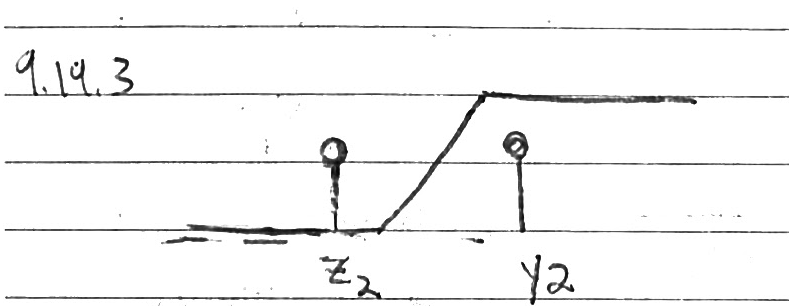
\includegraphics[width=0.5\textwidth]{figures/9-19-3.png}
    \end{center}
    \caption{Example of a ramp function to show necessity that $y_2 \leq z_2$.
      The ramp function should be drawn to be convex (i.e. continue increasing)}
  \end{figure}
  $g$ is convex and we see $\ex[g(Z)] = 0 \not\geq \ex[g(Y)]$

  \todo{Sufficiency}
\end{proof}

\subsection{Ledoux-Talagrand inequality}%

\myref{thm:ledoux-talagrand} is a statement involving maxima of randomly signed
sums of Lipschitz functions.
We saw an incomplete presentation in \cref{ssec:ledoux-talagrand-first} and
today will give the complete proof.

\begin{theorem}[Ledoux-Talagrand]\label{thm:ledoux-talagrand}
  Let $\phi : \RR \to \RR$ $L$-Lipschitz, $\phi(0) = 0$,
  $\{\eps_i\}_{i=1}^n \simiid \Rad$, $T =$ set of $n$-tuples $(t_1,\ldots,t_n)$
  (think $t_i = \braket{X_i - \mu, v}$). Then
  \begin{align}
    \ex\left[g \left(
        \sup_{t \in T} \sum_{i=1}^n \eps_i \phi(t_i)
    \right)\right]
    &\leq \ex\left[
      g\left(
        \sup_{t \in T} L \sum_{i=1}^n \eps_i t_i
      \right)
    \right]
  \end{align}
  for all convex increasing $g$.
\end{theorem}

In terms of stochastic dominance, this is saying that the random variables
\begin{align}
  Y &= \sup_{t \in T} \sum_{i=1}^n \eps_i \phi(t_i) \\
  Z &= \sup_{t \in T} L \sum_{i=1}^n \eps_i t_i
\end{align}
satisfy the second order stochastic dominance $Z \succeq Y$.
This means that $Z$ is more ``spread out'' than $Y$, which makes sense because
$\lvert \phi(s) - \phi(t) \rvert \leq L \lvert s - t \rvert$.

Another way to get this intutiion is to notice that the term inside the
supremum (for $L = 1$, if $\eps_i$ were Gaussian)
\begin{align}
  \Var\left(\sum_{i} \eps_i \phi(t_i)\right)
  &= \sum_i \phi(t_i)^2
  \leq \sum_{i} \lvert t_i \rvert^2
  = \Var\left(\sum_i \eps_i t_i\right)
\end{align}
So we would expect $Z$ to be more ``spread out'' because it has greater
variance.

We will prove the theorem for $n=2$ and then generalize by induction.

\begin{proof}[Proof for $n=2$]
  Let $T$ be the set of pairs $(a,b)$, $\phi$ be $1$-Lipschitz.
  Need to show
  \begin{align}
    \ex_\eps\left[
      g\left(
        \underbrace{\sup_{(a,b) \in T} a + \eps \phi(b)}_{\eqqcolon Y}
      \right)
    \right]
    &\leq
    \ex_\eps\left[
      g\left(
        \underbrace{\sup_{(a,b) \in T} a + \eps b}_{\eqqcolon Z}
      \right)
    \right]
  \end{align}
  Let $(a_+, b_+)$ be the maximizer of $a + \phi(b)$, and
  $(a_-, b_-)$ the maximizer of $a - \phi(b)$. Then
  \begin{align}
    \Pr[Y = y_1 = a_+ + \phi(b_+)] &= 1/2 \\
    \Pr[Y = y_2 = a_- - \phi(b_-)] &= 1/2 \\
    \Pr[Z = z_1 = \max(a_+ + b_+, a_- + b_-)] &= 1/2 \\
    \Pr[Z = z_2 = \max(a_- - b_-, a_+ + b_-+)] &= 1/2
  \end{align}

  \begin{figure}[H]
    \begin{center}
      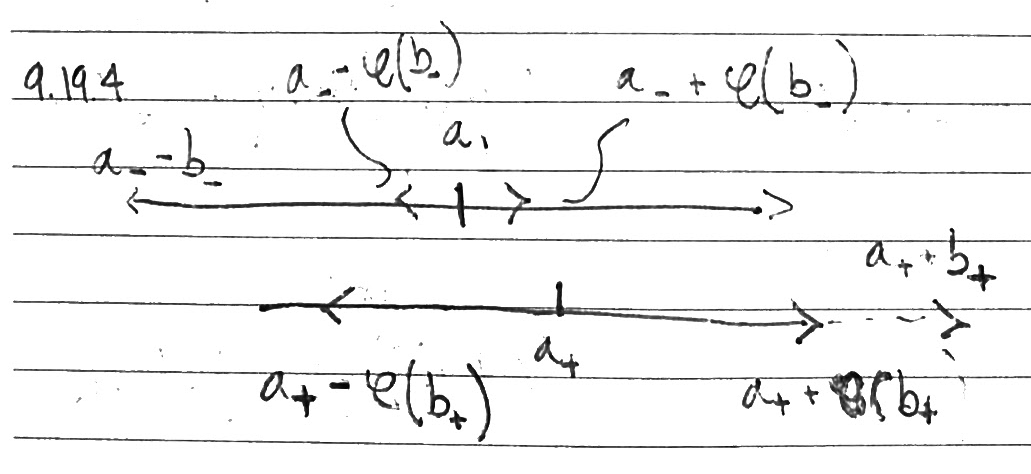
\includegraphics[width=0.5\textwidth]{figures/9-19-4.png}
    \end{center}
  \end{figure}

  By Lipschitz condition and definition of $y_i$, $z_i$:
  \begin{align}
    \max(y_1, y_2) &\leq \max(z_1, z_2) \\
    \max(a_+ + \phi(b_+), a_- - \phi(b_-))
                   &\leq \max(a_+ + \lvert b_+ \rvert, a_- + \lvert b_- \rvert) \\
    y_1 + y_2 &\leq z_1 + z_2 \\
    a_+ + a_- + \phi(b_+) - \phi(b_-)
              &\leq a_+ + a_- + \lvert b_+ - b_- \rvert
  \end{align}
  By \cref{lem:two-point-2o-sd}, we are done.
\end{proof}

\begin{proof}[Extending to $n > 2$]
  \begin{align}
    \ex_{\eps_{1:n}}\left[
      g \left(
        \sup_{t \in T} \sum_{i=1}^n \eps_i \phi(t_i)
      \right)
    \right]
    &=
    \ex_{\eps_{1:n-1}} \left[
      \ex_{\eps_{n}}\left[
        g \left(
          \sup_{t \in T} \underbrace{\sum_{i=1}^{n-1} \eps_i \phi(t_i)}_{a} + \eps_n \phi(\underbrace{t_n}_{b})
        \right)
      \middle\vert \eps_1,\ldots, \eps_{n-1} \right]
    \right] \\
    &\leq
    \ex_{\eps_{1:n-1}} \left[
      \ex_{\eps_{n}}\left[
        g \left(
          \sup_{t \in T} \sum_{i=1}^{n-1} \eps_i \phi(t_i) + \eps_n t_n
        \right)
      \middle\vert \eps_1,\ldots, \eps_{n-1} \right]
    \right] \\
    &=
    \ex_{\eps_{1:n}} \left[
      g \left(
        \sup_{t \in T} \sum_{i=1}^{n-1} \eps_i \phi(t_i) + \eps_n t_n
      \right)
    \right] \\
    &=
    \ex_{\eps_{[n] \setminus \{n-1\}}} \left[
        \ex_{\eps_{n-1}}\left[
          g \left(
            \sup_{t \in T} \sum_{i \in [n] \setminus \{n-1, n\}} \eps_i \underbrace{\phi(t_i) + \eps_n t_n }_{a}
            + \underbrace{\eps_{n-1} \phi(t_{n-1})}_{b}
          \right)
        \middle\lvert \eps_{[n] \setminus \{n-1\}} \right]
      \right]
  \end{align}
\end{proof}


\subsection{Bounding the empirical mean deviation}

We now return to bounding $\|\mu(p_n^*) - \mu(p^*)\|_2$, which is the other
step required before we can apply \cref{prop:projection-bound-expand-G-to-M}
for expanding the set.

The problem we encountered last time was the presence of a norm:
\begin{align}
  \ex[ \|\hat{\mu}_n - \mu\|_2^k ]
  &= \ex \left[ \left\| \frac{1}{n} \sum_{i=1}^n (X_i - \mu)\right\|_2^k \right]
\end{align}
One way to handle the norm is to take a supremum over inner products with
$v \in \cS^{d-1}$, since $\|w\|_2 = \sup_{v \in \cS^{d-1}} \braket{w,v}$.
Another is to use decoupling, which we will demonstrate today.

\textbf{Decoupling technique}: Use Khintchine's inequality to add in
an $\ex_\eps$ with one $\eps_i$ per dimension $d$.
Contrast this to symmetrization, which would have added random sign variables
across $n$ (one for each pair $(X_i, X_i')$).

\begin{lemma}[Khintchine's inequality]\label{lem:khintchine}
  Let $\eps = (\eps_1, \ldots, \eps_n) \simiid \Rad$.
  \begin{align}
    A_k \|Z\|_2 \leq \ex_\eps[\lvert \braket{\eps,z}\rvert^k]^{1/k} \leq B_k \|Z\|_2
  \end{align}
  with $A_k = \Theta(1)$ and $B_k = \Theta(\sqrt{k})$ if $k \geq 1$.
\end{lemma}

Applying the lower $\Theta(1)$ bound from \nameref{lem:khintchine}:
\begin{align}
  \ex_X [ \|\hat{\mu}_n - \mu\|_2^k ]
  &= \ex_X \left[ \left\| \frac{1}{n} \sum_{i=1}^n (X_i - \mu)\right\|_2^k \right] \\
  &\leq \cO(1)^k \ex_{X,\eps} \left[ \left\lvert \braket{\frac{1}{n} \sum_{i=1}^n (X_i - \mu), \eps} \right\rvert^k \right] \\
  &= \cO(1)^k \ex_{X, \eps}\left[
    \left\lvert
      \frac{1}{n} \sum^{n}_{i=1} \braket{X_i - \mu, \eps}
    \right\rvert^k
  \right]
\end{align}
Now pulling out the $n^{-k}$ and applying \ref{lem:rosenthal-ineq}
with $Z_i = \braket{X_i - \mu, \eps}$
\begin{align}
  \ex[\lvert \sum_i z_i \rvert^k]
  &\leq \cO(k)^k \sum_i \ex[\lvert Z_i \rvert^k]
  + \cO(\sqrt{k})^k \left(\sum_i \ex[\lvert Z_i \rvert^2]\right)^{k/2}
\end{align}
Under bounded $k$th moments hypothesis, $\ex[\lvert \braket{X - \mu,
v}\rvert^k] \leq \sigma^k \|v\|_2^k$ so
\begin{align}
  \ex[\lvert Z_i \rvert^k]
  &= \ex_{X,\eps}[\lvert \braket{X_i - \mu, \eps}\rvert^k]
  \leq \ex_\eps[\|\eps\|_2^k \sigma^k]
  = d^{k/2} \sigma^k
\end{align}

To record a tighter bound (since typically $\sigma_k \approx \sqrt{k} \sigma_2$),
let
\begin{align}
  \ex[\lvert \braket{X - \mu, v}\rvert^k]
  &\leq \sigma_k^k \|v\|_2^k \\
  \ex[\lvert \braket{X - \mu, v}\rvert^2]
  &\leq \sigma_2^k \|v\|_2^2
\end{align}
So Rosenthal's inequality (and adding back $n^{-k}$) becomes
\begin{align}
  \ex[\|\hat{\mu}_n - \mu\|_2^k]
  &\leq \cO(1)^k \ex_{X, \eps}[\lvert \frac{1}{n} \sum^{n}_{i=1} \braket{X_i - \mu, \eps}\rvert^k] \\
  &\leq \cO(1/n)^k \left[
    \cO(k)^k n d^{k/2} \sigma_k^k + \cO(\sqrt{k})^k (n d^{1/2} \sigma_2^2)^{k/2}
  \right] \\
  &= \cO\left(
    \left( \frac{k \sqrt{d}}{n} \sigma_k\right)^k n
    + \left(\sqrt{\frac{k d}{n}}\sigma_2 \right)^k
  \right)
\end{align}
In the case $\sigma_k = \sqrt{k} \sigma_2$, the second term dominates as long
as $n \geq k^{2k / (k-2)}$.

\textbf{Takeaway}: The average deviation $\ex[\|\hat{\mu}_n - \mu\|_2^k]^{1/k} \approx \cO(\sqrt{k d / n} \sigma_2)$.


\subsection{Zooming out}

\textbf{Goal}: we want the following to concentrate
\begin{align}
  \ex\left[\left\lvert
      \sup_{\|v\|_2 \leq 1} \frac{1}{n} \sum_{i=1}^n \left(
        \tilde{\psi}_k\left(\left\lvert
            \frac{\braket{X_i - \mu, v}}{\sigma}
          \right\rvert\right)
      \right)
      - \mu_{\tilde{\psi}_k}(v)
    \right\rvert^k\right]
\end{align}

By symmetrization
\begin{align}
  \ex\left[\left\lvert
      \sup_{\|v\|_2 \leq 1} \frac{1}{n} \sum_{i=1}^n \left(
        \eps_i \tilde{\psi}_k\left(\left\lvert
            \frac{\braket{X_i - \mu, v}}{\sigma}
          \right\rvert\right)
      \right)
    \right\rvert^k\right]
\end{align}

By Ledoux with $g(x) = x^k$
\begin{align}
  \ex\left[\left\lvert
      \sup_{\|v\|_2 \leq 1} \frac{1}{n} \sum_{i=1}^n \left(
        \eps_i \frac{(X_i - \mu)}{\sigma}
      \right)
    \right\rvert^k\right]
\end{align}
By a stronger version of the mean deviation inequality we just proved
